\subsection{Reduced Order Observer}
It has been decided to implement a reduced order observer, to observer the angular velocities. In general an observer is utilized in a control system if either one of two specific cases occurs. If certain states in the system are not measured, an observer can estimate the unmeasured states by the means of some of the measured state-variables. However, it is also possible to use an observer if the measured data gathered from the sensors is affected a significant amount of noise. As the observer in addition to estimating unmeasured states, also filters measurements \fxnote{feedback control of dynamic systems page 515}. The latter is however not focus more on in the prototype.

As explained earlier, the attitude model has six states, the three angles of the quadcopter (roll, pitch and yaw) and the three angular velocities. By using the Vicon system, the three angles of the quadcopter are measured, making it possible to estimate the angular velocities. With this approach, the first three states (angles), $x_1$ will be equal to the outputs, $y$, whereas the other three states will be estimated (angular velocities), $\hat{x}_2$.

In \autoref{fig:Observerdiagram1} a diagram illustrating the setup of the angular controller is shown. The highlighted lines is the reduced order observer and its corresponding inputs and output.
%
\begin{figure}[H]
    \includegraphics[scale=.4]{figures/ObserverColorDiagram}
    \centering			
    \captionof{figure}{An overall block diagram of the angular controller highlighting the reduced order observer and its corresponding inputs and output.}
    \label{fig:Observerdiagram1}
\end{figure}
%
The matrices which define the system can be separated into submatrices, which will be used in the design of the observer:\\
%
\begin{minipage}{0.45\linewidth}
    \begin{flalign}
        \vec{A}=
        \begin{bmatrix}
            \ \vec{A11}_{3 \times 3}  & \vec{A12}_{3 \times 3}    \ \ \ \\ 
            \ \vec{A21}_{3 \times 3}  & \vec{A22}_{3 \times 3}    \ \ \  		
        \end{bmatrix} \nonumber
    \end{flalign}
\end{minipage}   \hfill 
\begin{minipage}{0.45\linewidth}
    \begin{flalign}
        \vec{B}=
        \begin{bmatrix}
            \ \vec{B1}_{3 \times 4}    \ \ \ \\ 
            \ \vec{B2}_{3 \times 4}     \ \ \  		
        \end{bmatrix} \nonumber
    \end{flalign}
\end{minipage}\hfill
%\begin{minipage}{0.33\linewidth}
%    \begin{flalign}
%        \vec{C}=
%        \begin{bmatrix}
%            \ \vec{C}_{3 \times 3}  & \vec{0}_{3 \times 3}  \ \ \  		
%        \end{bmatrix} \nonumber
%    \end{flalign}
%\end{minipage}


As described before the system is observable. It is thereby possible to utilize the reduced order observer theorem \fxnote{The reduced order observer theorem slide 6 course 4 control.}. This theorem states, that for an observable system there always exist an gain $L_{obs}$ which ensures that \autoref{eq:observerStable} is stable.
%
\begin{flalign}
	\vec{A_{22}} + \vec{L_{obs}}\vec{A_{12}}
		\label{eq:observerStable}
\end{flalign}
%
The theorem also states that with this observer gain, the observer in \autoref{eq:eqobservertheorem} ensures that the estimate, $\hat{x}_2$, converges to $x_2$ with a rate yielded by the eigenvalues of \autoref{eq:eqobservertheorem}.
%
\begin{flalign}
	\vec{\hat{\dot{x}}_2} &= \vec{A_{21}}\vec{y} + \vec{A_{22}}\vec{\hat{x}_2} + \vec{B_2u} + \vec{L_{obs}}\vec{(A_{12}\hat{x}_2} - \vec{A_{21}x_2})
		\label{eq:eqobservertheorem}
\end{flalign}
%
To calculate an appropriate observer gain, $L_{obs}$, it is necessary to evaluate the reliability of the utilized sensor. If the gain is set very high, the estimation will rely more on the actual measurements of the outputs, whereas if it is very low, there will be more influence of the model in the final calculations \fxnote{christoffer slide 35 course 3}.

%The matrix in \autoref{Matrix:Lobs} is the decided observer gains utilized in the reduced order observer.
%
%\begin{flalign}
%	\vec{L_{obs}} = 
%	\begin{bmatrix}
%	\ -50 & 0 & 0  \ \ \ \\ 
%	\ 0 & -60 & 0  \ \ \ \\ 
%	\ 0 & 0 & -70  \ \ \  
%	\end{bmatrix}
%	\label{Matrix:Lobs}
%\end{flalign}

With the final design, \autoref{eq:eqobserverderived} shows how to estimate $\hat{x}_2$.
%
\begin{flalign}
    \vec{\hat{\dot{x}}_2} + \vec{L\dot{y}} &= \vec{(A_{22}} + \vec{LA_{12})\hat{x}_2} + \vec{(A_{21}} + \vec{LA_{11})y} + (\vec{B_2} + \vec{LB_1})\vec{u}
    \label{eq:eqobserverderived}
\end{flalign}
%
This estimation can also be seen in the form of a block diagram, \autoref{fig:observerDiagram}.
\begin{figure}[H]
	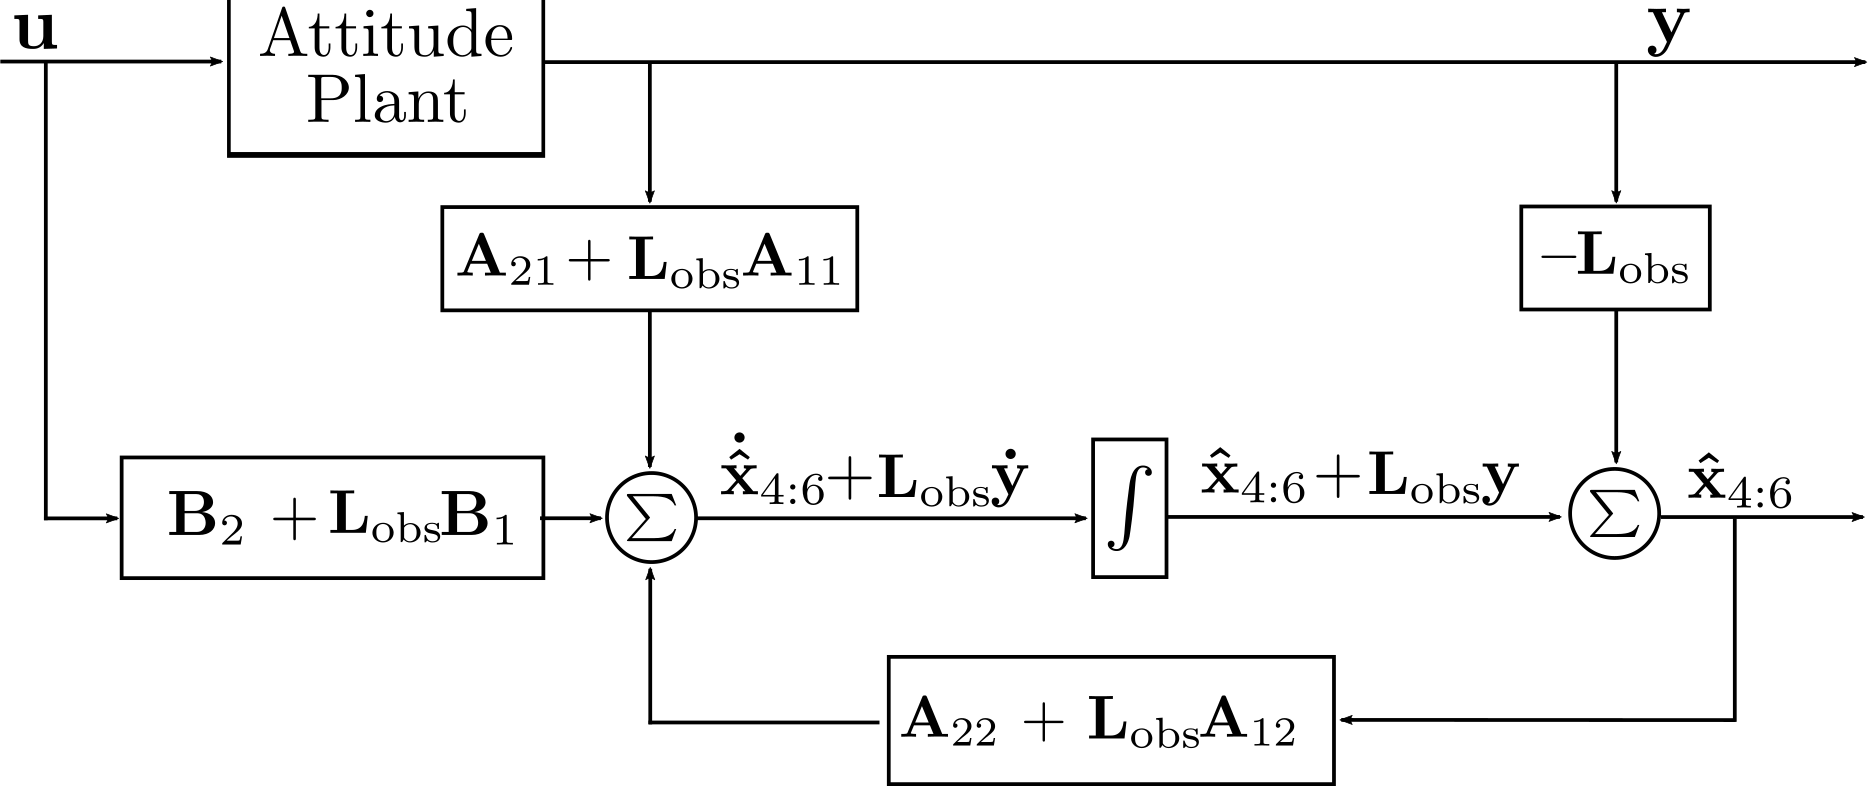
\includegraphics[scale=.35]{figures/observerDiagram}
	\centering
	\captionsetup{justification=centering}
	\captionof{figure}{A diagram showing the reduced order observer and how it is implemented.}
	\label{fig:observerDiagram}
\end{figure}











%\begin{minipage}{0.15\linewidth}
%	\begin{flalign}
%	A_{11} = 
%	\begin{bmatrix}
%		\ 0 & 0 & 0 \ \ \\ 
%		\ 0 & 0 & 0 \ \ \\ 
%		\ 0 & 0 & 0 \ \ \\
%	\end{bmatrix}	\nonumber
%	\label{A11}
%	\end{flalign}  
%\end{minipage}\hfill
%\begin{minipage}{0.15\linewidth}
%	\begin{flalign}
%	A_{12} = 
%	\begin{bmatrix}
%		\ 1 & 0 & 0 \ \ \\ 
%		\ 0 & 1 & 0 \ \ \\ 
%		\ 0 & 0 & 1 \ \ \\
%	\end{bmatrix}	\nonumber
%	\label{A12}
%	\end{flalign}
%\end{minipage}\hfill
%\begin{minipage}{0.15\linewidth}
%	\begin{flalign}
%	A_{21} = 
%	\begin{bmatrix}
%		\ 0 & 0 & 0 \ \ \\ 
%		\ 0 & 0 & 0 \ \ \\ 
%		\ 0 & 0 & 0 \ \ \\
%	\end{bmatrix}	\nonumber
%	\label{A21}
%	\end{flalign}
%\end{minipage}\hfill
%\begin{minipage}{0.15\linewidth}
%	\begin{flalign}
%	A_{22} = 
%	\begin{bmatrix}
%		\ 0 & 0 & 0 & 0 \ \ \\ 
%		\ 0 & 0 & 0 & 0 \ \ \\ 
%		\ 0 & 0 & 0 & 0 \ \ \\
%	\end{bmatrix} \nonumber
%	\label{A22}
%	\end{flalign}
%\end{minipage}\hfill
%
%
%\begin{minipage}{0.4\linewidth}
%	\begin{flalign}
%	B_1 = 
%	\begin{bmatrix}
%		\ 0 & 0 & 0 & 0 \ \ \\ 
%		\ 0 & 0 & 0 & 0 \ \ \\ 
%		\ 0 & 0 & 0 & 0 \ \ \\
%	\end{bmatrix}	\nonumber
%	\label{B1}
%	\end{flalign}
%\end{minipage}\hfill
%\begin{minipage}{0.6\linewidth}
%	\begin{flalign}
%	B_2 = 
%	\begin{bmatrix}
%		0 & \si{-\frac{2 \  k_{th} \  L \  \overline{\omega}_2}{J_x}} & 0 & \si{\frac{2 \  k_{th} \  L \  \overline{\omega}_4}{J_x}} \ \ \ \\ 
%		\ \si{\frac{2 \  k_{th} \  L \  \overline{\omega}_1}{J_y}} & 0 & \si{-\frac{2 \  k_{th} \  L \  \overline{\omega}_3}{J_y}} & 0 \ \ \ \\ 
%		\frac{2 \  k_d \  {\overline{\omega}_1}}{J_z} & - \frac{2 \  k_d \  {\overline{\omega}_2}}{J_z} & \frac{2 \  k_d \  {\overline{\omega}_3}}{J_z} & - \frac{2 \  k_d \  {\overline{\omega}_4}}{J_z} \ \ \
%	\end{bmatrix} \nonumber
%	\label{B2}
%	\end{flalign}
%\end{minipage}\hfill
%
%
%\begin{flalign}
%	L_{obs} = 
%	\begin{bmatrix}
%	\ -50 & 0 & 0  \ \ \ \\ 
%	\ 0 & -60 & 0  \ \ \ \\ 
%	\ 0 & 0 & -70  \ \ \  
%	\end{bmatrix}
%	\label{Lobs}
%\end{flalign}


